% ============================================================
% ダイオードを用いた電子回路 本文
% 担当の先生はこのファイルと figures/ だけを編集してください。
% 図のラベルは fig:diode-○○ の形にしてください（他テーマとの重複防止）。
% ============================================================
\graphicspath{{contents/03_diode/figures/}}

\experimenttitle{ダイオードを用いた電子回路}

% ============================================================
\section{目的}

発光ダイオード（LED：Light Emitting Diode）の整流性を確認し，発光色の異なるLEDの点灯と電圧の関係を調べます。また，ダイオードの整流性を利用した整流回路について出力波形の変化を調べます。

% ============================================================
\section{ダイオードについて}

ダイオードは，電流を一方向にのみ流す電子部品です。電気の流れをコントロールする「電気の逆流防止弁」のような働きをします。ダイオードは，P型半導体とN型半導体が接合した構造をしており，この接合面をPN接合と呼びます。

\begin{figure}[htbp]
  \centering
  \begin{minipage}[b]{0.46\linewidth}
    \centering
    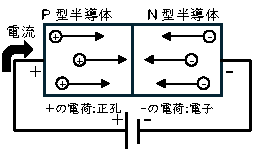
\includegraphics[scale=1.3]{diode_pn_forward.pdf}
    \caption{順方向電圧を印加}
    \label{fig:diode-pn_forward}
  \end{minipage}
  \hfill
  \begin{minipage}[b]{0.46\linewidth}
    \centering
    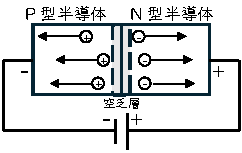
\includegraphics[scale=1.3]{diode_pn_reverse.pdf}
    \caption{逆方向電圧を印加}
    \label{fig:diode-pn_reverse}
  \end{minipage}
\end{figure}

図\ref{fig:diode-pn_forward}に示すように，P型半導体側にプラス，N型半導体側にマイナスの電圧（順方向電圧）を印加すると，PN接合部分で，正の電荷（正孔）と負の電荷（電子）が再結合して電流が流れます。一方，図\ref{fig:diode-pn_reverse}に示すようにP型半導体側にマイナス，N側半導体側にプラスの電圧（逆方向電圧）を印加するとPN接合の部分に電荷が存在しない空乏層が形成され，電流は流れません。この性質を利用して，様々な電子機器に利用されています。

\subsection{ダイオードの種類}

ダイオードには様々な種類があり，それぞれ異なる用途で使用されています。

\begin{enumerate}
  \item \keyword{発光ダイオード（LED）}\quad ※本実験では，LEDを用いた実験を行います。\\
    順方向に電圧を印加すると発光します。LEDの材料によって，発光色や光り始める電圧が異なります。信号機，照明，ディスプレイなど，現代の生活に欠かせない部品の1つです。
  \item \keyword{整流ダイオード}\\
    交流を直流に変換する整流回路に特化した素子です。LEDよりも大きな電流を扱うことができ，家電製品の電源回路など，幅広い電子機器で使用されています。
  \item \keyword{ツェナーダイオード}\\
    逆方向に一定以上の電圧（ツェナー電圧）を印加しても電流が流れる性質を持ちます。電圧を一定に保つ定電圧回路に使用されます。
  \item \keyword{フォトダイオード}\\
    光を受けると電流を流す受光素子で，光センサー等に使用されます。出力電力に特化したものが太陽電池になります。
\end{enumerate}

\subsection{LED}

\begin{figure}[htbp]
  \centering
  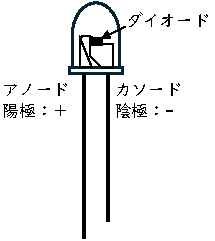
\includegraphics[scale=1.3]{diode_led_appearance.pdf}
  \caption{LEDの外観図}
  \label{fig:diode-led}
\end{figure}

図\ref{fig:diode-led}に砲弾型のLEDの外観図を示します。金属線が長いほうがアノード（陽極：$+$），足が短いほうがカソード（陰極：$-$）となります。金属線の長さに違いがない場合は，LEDの発光部を横から見て判別します。ダイオードが乗っていない側（図\ref{fig:diode-led}では左側）がアノード，ダイオードが乗っている側（図\ref{fig:diode-led}では右側）がカソードとなります。LEDに順方向電圧を印加するとPN接合の部分で正孔と電子が再結合して電流が流れて発光します。LEDの発光色は使用されているダイオードの材料によって異なります。赤色にはアルミニウムガリウムヒ素（AlGaAs）やガリウムヒ素リン（GaAsP）など，黄緑色には窒化インジウムガリウム（InGaN）など，青色には窒化ガリウム（GaN）などが用いられています。

% ============================================================
\section{使用器具}

\begin{equipment}
\begin{itemize}
  \item LED（赤色6個，黄緑色1個，青色1個，白色1個）\quad ※接続時，極性（向き）に注意
  \item 固定抵抗器 $R$（\SI{100}{\ohm}/\SI{1}{W}，\SI{1}{\mega\ohm}/\SI{0.25}{W}）\quad ※極性（向き）はありません
  \item セラミックコンデンサー $C$（\SI{10}{\micro F}）1個\quad ※極性（向き）はありません
  \item ブレッドボード 1個
  \item ジャンパー線 必要数
  \item 直流電源 1台\quad ※接続時，極性（向き）に注意
  \item 交流電源 1台\quad ※接続時，極性（向き）に注意
  \item オシロスコープ 1台
  \item オシロスコープのプローブ 2本
\end{itemize}
\end{equipment}

% ============================================================
\section{実験方法}

% ------------------------------------------------------------
\subsection{実験1：LEDの整流性の確認と赤色LEDの点灯実験}

赤色LEDの整流性を確認するため，逆方向接続もしくは順方向接続して電圧印加時の赤色LEDの点灯状態を確認します。

\begin{figure}[htbp]
  \centering
  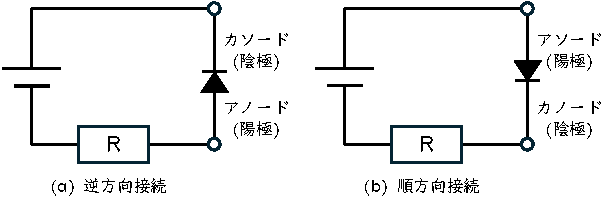
\includegraphics[scale=1.3]{diode_exp1_circuit.pdf}
  \caption{実験1の回路図}
  \label{fig:diode-exp1}
\end{figure}

\begin{procedure}[label=\textbf{(\alph*)}]
  \item \keyword{逆方向接続}\\
    LEDの極性（アノードとカソードの向き）に気を付けて，逆方向電圧を印加する回路をブレッドボード上に作製します（図\ref{fig:diode-exp1}(a)逆方向接続）。固定抵抗器 $R$（\SI{100}{\ohm}/\SI{1}{W}）は，LEDに電流が流れすぎないようにするために用います。出力をONした後，直流電源の電圧を\SI{0}{V}から\SI{3}{V}（実際には直流電源を逆に接続するため回路には\SI{0}{V}から\SI{-3}{V}）までゆっくりと印加し，直流電源に表示される電流と赤色LEDの発光状態を確認します。\wave{発光しないことを確認後，電圧を\mbox{\SI{0}{V}}にもどし，出力をOFFします。}
  \item \keyword{順方向電圧}\\
    LEDの極性に気を付けて，順方向電圧を印加する回路をブレッドボード上に作製します（図\ref{fig:diode-exp1}(b)順方向接続）。出力をONした後，直流電源の電圧を\SI{0}{V}からゆっくりと印加し，直流電源に表示される電流表示が\SI{0.001}{A}となるときの電圧 $V$（V）を読み取り，課題1の表に記載します。\wave{発光確認後，電圧を\mbox{\SI{0}{V}}にもどし}，\wave{出力をOFFします。}
\end{procedure}

% ------------------------------------------------------------
\subsection{実験2：様々なLEDの点灯実験}

異なる色のLEDが点灯する電圧（電流表示が\SI{0.001}{A}になる）を調べます。

LED（黄緑色LED，青色LED，白色LED）の極性に気を付けて順方向電圧を印加する回路をブレッドボード上に作製します（図\ref{fig:diode-exp1}(b)順方向接続）。出力をONした後，直流電源の電圧を\SI{0}{V}からゆっくりと印加し，電源電圧の電流表示が\SI{0.001}{A}となるとき，各LEDの電圧 $V$（V）を読み取り，課題1の表に記載します。\wave{発光確認後，電圧を\mbox{\SI{0}{V}}にもどし}，\wave{出力をOFFします。}
% TODO(原文確認): 次の文は原文のまま。意味が通らないため要修正
\wave{LEDを交換し，}\wave{電圧の出力とで電圧に気を付けLEDが点灯する電圧を調べます。}

% ------------------------------------------------------------
\subsection{実験3：赤色LEDの整流性を利用した電圧波形の変化}

LEDの整流性を利用し，正弦波交流波形の変化を観測します。

\subsubsection{オシロスコープの準備}

\begin{procedure}
  \item オシロスコープに電源ケーブルを接続し，主電源を入れてオシロスコープが起動するのを待ちます。
  \item 起動後，「Default Setup」ボタンを押し，オシロスコープの設定を初期化します。初期化によって電圧軸は\SI{5.00}{V}/DIV，時間軸は\SI{100.0}{\micro s}/DIVに設定されます。
  \item CH1にオシロスコープのプローブを接続し，CH1の測定端子をオシロスコープのDemo端子に接続します。
  \item 「Auto Scale」ボタンを押すと，電圧軸は\SI{500}{mV}/DIV，時間軸は\SI{200.0}{\micro s}/DIVに設定され，Demo端子からの波形が表示されます。
  \item 「Meas」ボタンを押すと，Demo端子からの出力波形の周波数がおよそ\SI{1}{kHz}，p-pがおよそ\SI{2.5}{V}であることがわかります。
  \item オシロスコープのCH1とCH2の接続部分の上部に記載されています「押してゼロ設定」の「右側のノブ」を押すと，基準電圧が中央に移動します。
  \item 垂直軸をまわして電圧を\SI{2.00}{V}/DIV，水平軸をまわして時間を\SI{200.0}{ms}/DIVに設定します。
\end{procedure}

\subsubsection{交流電源の準備}

\begin{figure}[htbp]
  \centering
  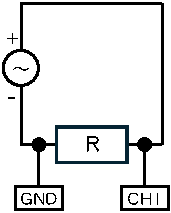
\includegraphics[scale=1.3]{diode_ac_setup.pdf}
  \caption{交流電源設定回路}
  \label{fig:diode-ac_setup}
\end{figure}

\begin{procedure}
  \item 交流電源に電源ケーブルを接続し，出力ケーブルを接続します。
  \item 交流電源のAMPLが最小値（反時計回りに回りきっている状態），ATTが押されていない状況を確認し，交流電源をONします。
  \item 周波数を\SI{2}{Hz}（x20のボタンを押し，\SI{0.0020}{kHz}表示），正弦波形のボタンを押します。
  \item ブレッドボード上に図\ref{fig:diode-ac_setup}の回路（固定抵抗 $R$（\SI{100}{\ohm}/\SI{1}{W}））を作製し，オシロスコープのCH1のプローブを図\ref{fig:diode-ac_setup}のように接続します。
  \item 交流電源のAMPLをゆっくりと増加（時計回りに回す）させ，オシロスコープのp-pがおよそ\SI{12.0}{V}となるように設定し，「トリガ」を回し，トリガの位置を\SI{2.00}{V}にします。
  % 原文はSymbolフォントで「200 μs/DIV」。2 Hzの観測なので ms と判断（要確認）
  \item オシロスコープで観察される電圧波形を課題2の図(a)に図示してください。（オシロスコープの表示設定は\SI{2.00}{V}/DIV，\SI{200}{ms}/DIVとなっています。）
  \item 観察終了後，交流電源の電源をOFFにします。
\end{procedure}

\subsubsection{LEDを用いた点灯実験}

\begin{figure}[htbp]
  \centering
  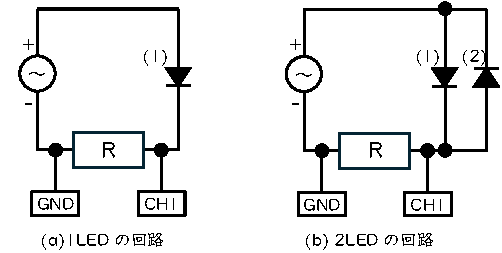
\includegraphics[scale=1.3]{diode_led_ac.pdf}
  \caption{LEDを用いた点灯実験}
  \label{fig:diode-led_ac}
\end{figure}

\begin{procedure}
  \item LEDの極性に気を付けて図\ref{fig:diode-led_ac}(a)に示す回路をブレッドボード上に作製します。
  \item オシロスコープのCH1のプローブを図\ref{fig:diode-led_ac}(a)のように接続したのち，交流電源をONにして，LED(1)の点灯状態とオシロスコープで抵抗器 $R$ の電圧波形を確認します。（LED(1)が点滅します。）
  \item 確認後，交流電源の電源をOFFにします。
  \item LEDの極性に気を付けて図\ref{fig:diode-led_ac}(b)に示す回路をブレッドボード上に作製します。
  \item 交流電源をONにして，LEDの点灯状態とオシロスコープで抵抗器 $R$ の電圧波形を確認します。（LED(1)とLED(2)が交互に点灯します。）
  \item 確認後，交流電源をOFFにします。
\end{procedure}

\subsubsection{整流回路1}

\begin{figure}[htbp]
  \centering
  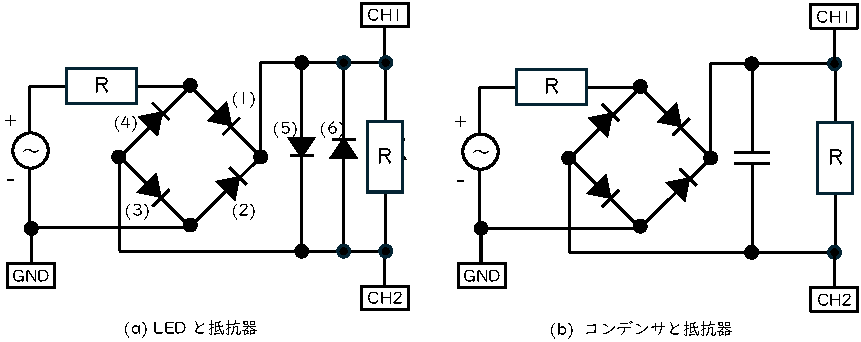
\includegraphics[width=0.95\linewidth]{diode_rectifier.pdf}
  \caption{整流回路}
  \label{fig:diode-rectifier}
\end{figure}

\begin{procedure}
  \item 図\ref{fig:diode-rectifier}(a)の回路をブレッドボード上に作製します。\wave{固定抵抗 \mbox{$R$} は\mbox{\SI{1}{\mega\ohm}}/\mbox{\SI{0.25}{W}}を使用します。}
  \item 交流電源をONにし，LEDの点灯状態を確認します。正電圧印加時にLED(1)，LED(3)，LED(5)が点灯し，負電圧印加時にLED(2)，LED(4)，LED(5)が点灯するため，正しく回路が接続されていれば，LED(1)，LED(3)，LED(5)とLED(2)，LED(4)，LED(5)が交互に点灯し，LED(6)は点灯しません。
  \item 確認後，交流電源の電源をOFFします。
  \item オシロスコープのCH1とCH2のプローブを図\ref{fig:diode-rectifier}(a)のように接続します。
  \item 「CH2」のボタンを押し，CH2を表示させ，CH2の電圧軸を\SI{2.00}{V}/DIVに設定します。
  \item 「Math」ボタンを押し，演算子を「$-$」に設定してCH1$-$CH2を表示させます。
  \item 「CH1」と「CH2」のボタンをそれぞれ2回押し，CH1とCH2の表示をOFFします。
  % 原文はSymbolフォントで「200 μs/DIV」。ms と判断（要確認）
  \item 交流電源をONして，オシロスコープで観察されるCH1$-$CH2のMathの電圧波形を課題2の図(b)に図示します。（オシロスコープの表示設定は\SI{2.00}{V}/DIV，\SI{200}{ms}/DIVのままです。）
  \item 図示後，交流電源をOFFします。
\end{procedure}

\subsubsection{整流回路2}

\begin{procedure}
  \item 図\ref{fig:diode-rectifier}(b)に示す回路をブレッドボード上に作製します。
  % 原文はSymbolフォントで「200 μs/DIV」。ms と判断（要確認）
  \item 交流電源をONにし，オシロスコープで観察されるCH1$-$CH2のMathの電圧波形を課題2の図(c)に図示します。（オシロスコープの表示設定は\SI{2.00}{V}/DIV，\SI{200}{ms}/DIVとします。）
  \item 図示後，交流電源をOFFにします。
\end{procedure}

\subsubsection{実験終了後}

\begin{procedure}
  \item オシロスコープの「Default Setup」ボタンを押し，オシロスコープの設定を初期化後，オシロスコープの電源をOFFします。
  \item オシロスコープと交流電源の電源ケーブルをはずします。また，実験に使用したLED，抵抗器，セラミックコンデンサーは袋にしまい，接続ケーブル等はプラスチックのケースに戻します。
\end{procedure}
